\chapter{Manual técnico}
\noindent
A pesar de que la plataforma web está actualmente disponible en:

\begin{center}
\textit{http://tec.citius.usc.es/stac/index.html},
\end{center}

\noindent
en este apéndice se muestra el manual de despliegue, pensado para que los usuarios puedan configurar y poner en funcionamiento la plataforma en sus equipos. Para ello, se tomará como base el Sistema Operativo Ubuntu 14.04, junto con Apache 2.4. Las razones de realizar el despliegue con Apache y no con el propio servidor de Bottle se detallan en la sección \ref{tecnologias}. En la figura \ref{fig:directorio_proy}, podemos ver los sub directorios que forman parte del directorio del proyecto:

\begin{figure}[H]
\centering
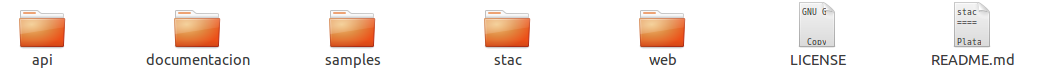
\includegraphics[scale=0.5]{figuras/directorio_proy.png}
\caption{Directorio del proyecto STAC.}
\label{fig:directorio_proy}
\end{figure}

\begin{itemize}
\item \textbf{api:} API REST (servicios web, archivo de la librería de Bottle y archivo app.wgi).
\item \textbf{documentación:} archivos de la memoria y documentación de los test estadísticos con Sphinx.
\item \textbf{samples:} muestras de ficheros de datos.
\item \textbf{stac:} módulo Python de los test estadísticos.
\item \textbf{web:} archivos web (Framework Bootstrap, CSS, JavaScript, imágenes, etc.).
\end{itemize}

\section{Despliegue de la aplicación en Apache}

\begin{enumerate}
\item Instalar Apache, el módulo WSGI y la librería SciPy:
\subitem - \texttt{sudo apt-get install apache2}
\subitem - \texttt{sudo apt-get install libapache2-mod-wsgi}
\subitem - \texttt{sudo apt-get install python-scipy}
\item Crear un enlace simbólico para enlazar el directorio del proyecto al directorio raíz de Apache y cambiar los permisos del directorio raíz \texttt{/var/www}:
\subitem - \texttt{sudo ln -s \$STAC /var/www/stac}
\subitem - \texttt{sudo chmod -R 755 /var/www}
\item El siguiente paso es cambiar la configuración de Apache para que el módulo WSGI cargue la API REST. Para ello se crea el archivo \texttt{/etc/apache2/sites-available/stac.conf} con el siguiente contenido:
\begin{lstlisting}
<VirtualHost *:80>
   ServerName stac
   ServerAlias stac
   
   DocumentRoot /var/www/stac/web
   
   <Directory /var/www/stac/web>
      Order deny,allow
      Allow from all
   </Directory>

   WSGIDaemonProcess stac user=www-data group=www-data processes=1 threads=1
   WSGIScriptAlias /api /var/www/stac/api/app.wsgi
   
   <Directory /var/www/stac/api>
      WSGIProcessGroup stac
      WSGIApplicationGroup \%{GLOBAL}
      Order deny,allow
      Allow from all
   </Directory>

</VirtualHost>
\end{lstlisting}
\item El módulo WSGI buscará el archivo \texttt{/var/www/stac/api/app.wsgi} para cargar la aplicación en el servidor web. El contenido de app.wsgi es el siguiente:
\begin{lstlisting}
import sys, os, bottle
from bottle import route, Bottle

sys.path = ['/var/www/api/'] + sys.path
os.chdir(os.path.dirname(__file__))

import servicios # Importa los servicios REST

application = bottle.default_app() # Carga la aplicacion por defecto con los servicios REST
root = Bottle()
root.mount('/api/', application) # Hacemos que todos los servicios escuchen en /api
\end{lstlisting}
\item Activar el sitio:
\subitem - \texttt{sudo a2ensite stac}
\item Desactivar el sitio por defecto si es necesario:
\subitem - \texttt{sudo a2disite 000-default}
\item Reiniciar servidor:
\subitem - \texttt{sudo service apache restart}
\end{enumerate}